\documentclass[a4paper,twoside,11pt]{article}
\usepackage{a4wide,graphicx,subfigure,fancyhdr,amsmath,amssymb,algpseudocode,enumerate,hyperref, float,placeins}
\usepackage[english]{babel}
\numberwithin{equation}{section}

%----------------------- Macros and Definitions --------------------------

\setlength\headheight{20pt}
\addtolength\topmargin{-10pt}
\addtolength\footskip{20pt}

\newcommand{\N}{\mathbb{N}}
\newcommand{\ch}{\mathcal{CH}}

\fancypagestyle{plain}{%
\fancyhf{}
\fancyhead[LO,RE]{\sffamily\bfseries\large}
\fancyhead[RO,LE]{\sffamily\bfseries\large }
\fancyfoot[LO,RE]{\sffamily\bfseries\large }
\fancyfoot[RO,LE]{\sffamily\bfseries\thepage}
\renewcommand{\headrulewidth}{0pt}
\renewcommand{\footrulewidth}{0pt}
}

\pagestyle{fancy}
\fancyhf{}
\fancyhead[RO,LE]{\sffamily\bfseries\large 2IN35}
\fancyhead[LO,RE]{\sffamily\bfseries\large Lab 3 }
\fancyfoot[LO,RE]{\sffamily\bfseries\large }
\fancyfoot[RO,LE]{\sffamily\bfseries\thepage}
\renewcommand{\headrulewidth}{1pt}
\renewcommand{\footrulewidth}{0pt}
\newcommand{\name}{VLSI Programming}

%-------------------------------- Title ----------------------------------

\title{\vspace{-\baselineskip}\sffamily\bfseries VLSI Lab 3}

\author{
Nicky Advokaat - 0740567 - {\tt n.advokaat@student.tue.nl} \\
Marcel  Moreaux - 0499480 - {\tt  m.l.moreaux@student.tue.nl}\\
}

\date{4\textsuperscript{rd} quartile, 2014}

%--------------------------------- Text ----------------------------------

\begin{document}
\maketitle
\thispagestyle{empty}
\begin{abstract}
This report contains solutions for the problems described in Assignment L3 for the course VLSI Programming. We will transform a parallel FIR filter to a sequential one to reduce hardware utilization. We will also create a strength reduced version of this filter.
\end{abstract}

\tableofcontents

\newpage

\section{Problem Specification and Requirements}
The goal of this assignment is to construct an upscaler that increases the sample rate of an input signal from 44.1 KHZ to 48 KHZ, which gives the upscaling ratio $\frac{160}{147}$.  This is done by first upscaling by L=160, then applying a filter, and the downscaling by M=147.  The coefficients for the filter are constructed from the \texttt{lanczos} function, which is a finite window version of the \texttt{sinc} function. We will have to generate these coefficients ourselves, and store them in ROM memory. There several alternatives to construct the upscaler, these are discussed in section ~\ref{sec:Q3}. The upscaler must have a clock frequency of at least 100 MHz. We have a choice whether to optimize the upscaler for minimum resource utilization, or for maximum throughput. After we have designed and implemented the upscaler we will test it by analyzing the input and output signals.

\section{Solution}
In this section we describe the key ideas behind our design, and the decisions we made during the design process.
\subsection{Sequential Implementation}
To implement a sequential filter we had to solve a number of problems. In between each data input, we have to do 32 multiply accumulate operations. Therefore we have to buffer the latest 32 input values in an array \texttt{data}, in which the 0th index contains $x(i)$ and the last value is $x(i -31)$. This can be seen at the top of figure ~\ref{fig:architecture}. So in each step, the new data value is supplied to \texttt{data}[0], and for all $1 \leq i \leq 31$ the value of \texttt{data}[$i$-1] is copied to \texttt{data}[$i$]. An alternative solution would be to create a ring buffer, in which we supply the input value to the $(n\bmod 32)$-th slot of \texttt{data}. We decided not to use this approach, because it would require an extra register to point to the latest variable, and an extra multiplexer to index the input wires of the array.\\
After the $n^{th}$ input is supplied we need to calculate $y(n)=\Sigma_{0\leq i \leq 31}(h(i)\cdot x(n-i))$. In our design this corresponds to $\Sigma_{0 \leq i \leq 31}(data[i] * h\_in[i])$.  

\begin{figure}
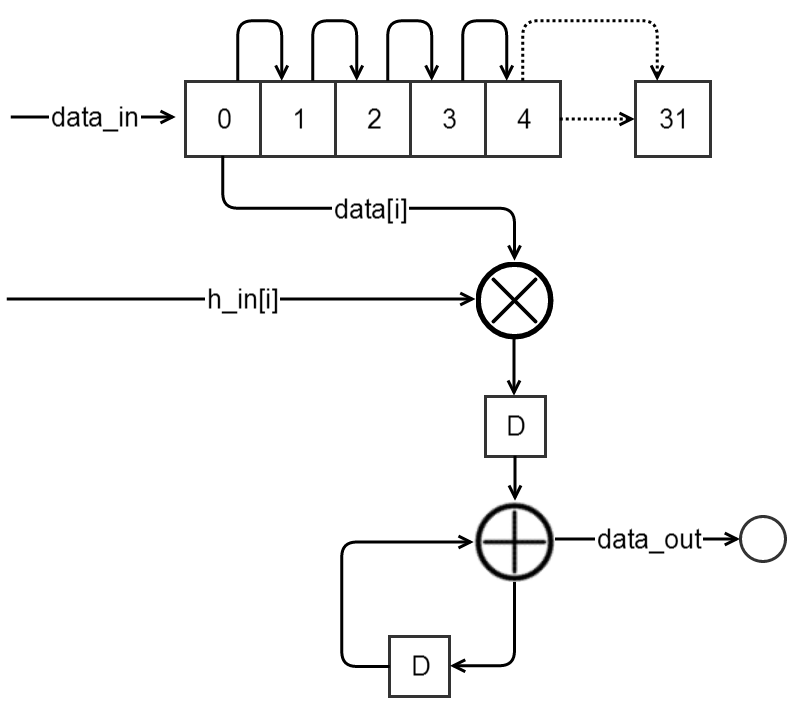
\includegraphics[width=0.9\textwidth]{images/architecture.png}
\caption{Architecture diagram of the sequential FIR filter.}
\label{fig:architecture}
\end{figure}


\section{Results}
\subsection{Resource Usage}
\subsection{Properties}
ISE report the following timing statistics for our design with $n$ = 1024. 
\begin{itemize}
\item
Synthesis report
\begin{itemize}
\item Minimum period: 14.714ns
\item Maximum Frequency: 67.961MHz
\end{itemize}
\item
Post-PAR static timing report
\begin{itemize}
\item  Minimum period:   16.155ns  
\item Maximum frequency: 61.900MHz
\end{itemize}
\end{itemize}
 This leaves us with a maximum frequency that is lower than 100 MHz. But because we produce output every clock cycle, we can still process 1024 streams at once. Therefore the 100 MHz requirement does not seem very important, it does however mean that we can not compile our design on the ngrid server. 
\subsection{Analysis of Filter Output }
\label{sec:analysis}
In this section we will show correctness of the upscaler by analyzing the input and output. Figure ~\ref{fig:plot1} shows the first part of the input and output signal. There is a finite amount of startup noise, indicated by the first part of the output signal being zero. It also shows the latency of the system, the output signal has some delay compared to the input signal. But except for those differences the signals appear identical.
\begin{figure}
\begin{center}
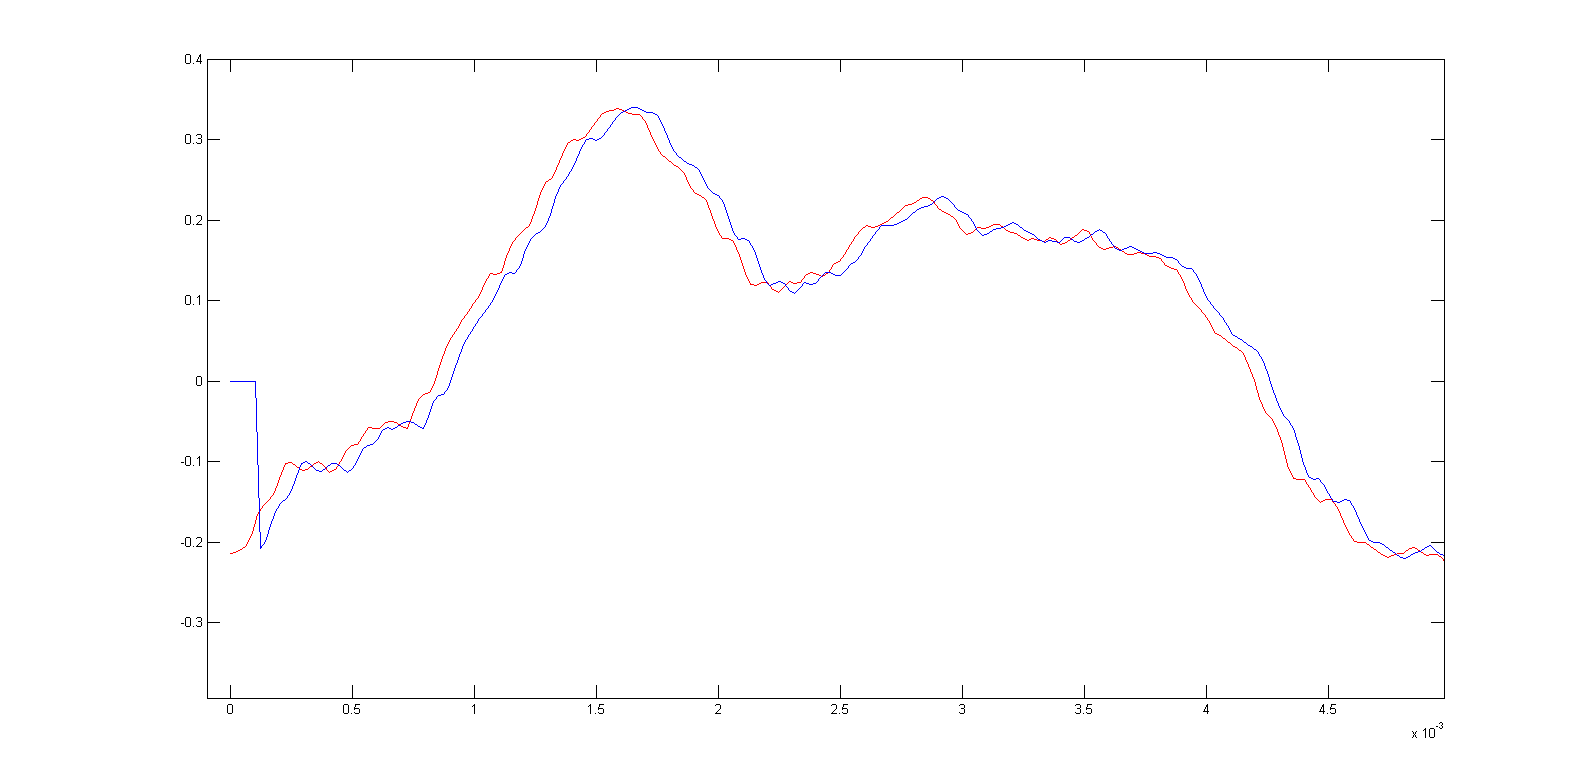
\includegraphics[width=0.7\textwidth]{images/plot1.png}
\caption{Plot of the first part of the original signal (red) and the signal after filtering (blue).}
\label{fig:plot1}
\end{center}
\end{figure}
In figure ~\ref{fig:plot2} we see another plot of the input and output signal. In this plot we have shifted the output signal by -3 samples, and there are dots indicating the samples. We can now see that the output signal has a higher sample frequency than the input signal. 
\begin{figure}
\begin{center}
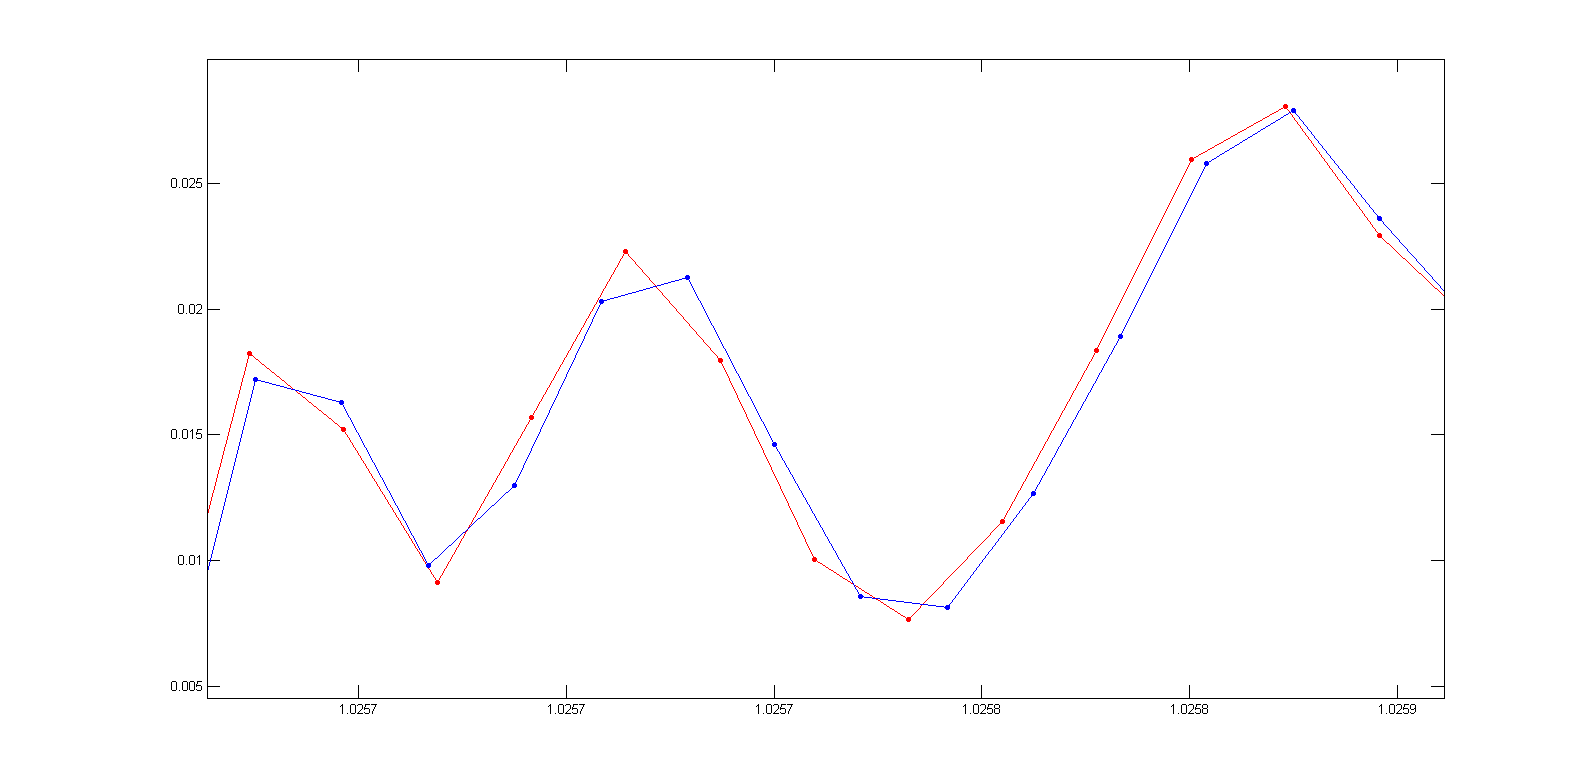
\includegraphics[width=0.7\textwidth]{images/plot2.png}
\caption{Plot of part of the original signal (red) and the signal after filtering (blue) with dots indicating the samples.}
\label{fig:plot2}
\end{center}
\end{figure}
\FloatBarrier
Figure ~\ref{fig:spectrum} shows the signals in the frequency domain. There is only minimal difference between them. The output frequency contains a higher maximum frequency because it has a higher sample rate. 
\begin{figure}
\begin{center}
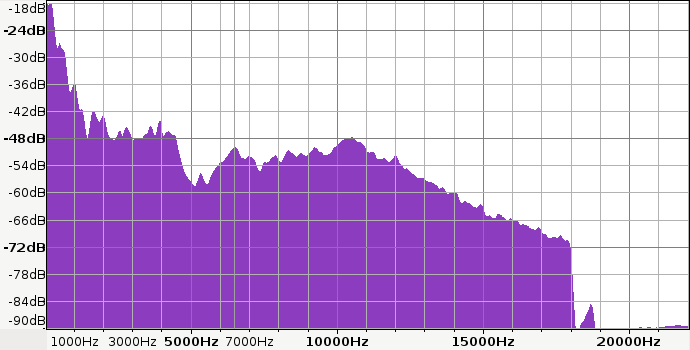
\includegraphics[width=0.7\textwidth]{images/freq1.png}
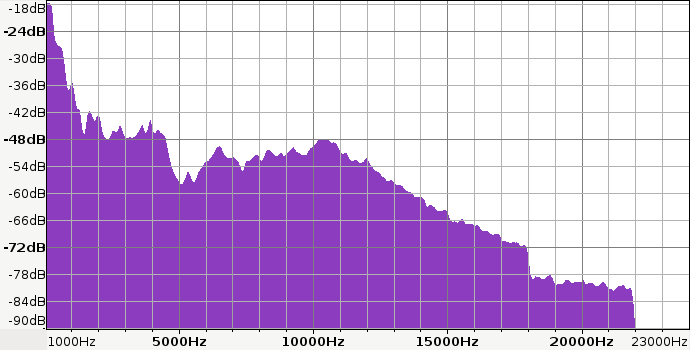
\includegraphics[width=0.7\textwidth]{images/freq2.png}
\caption{Plot in the frequency domain of the original signal (top) and the signal after filtering (bottom).}
\label{fig:spectrum}
\end{center}
\end{figure}
Finally, figure ~\ref{fig:wave} displays some waveforms of the design. For this image we have used $n = 2$. We can see this in the input and output streams, in which \texttt{$<$0000$>$} is interleaved with nonzero values. If we look at \texttt{clk} we can see that we do indeed produce output every clock cycle. We can also see a period in which \texttt{filter\_in\_ack} and \texttt{filter\_req\_ack} are zero, during which input and output remain stable.
\begin{figure}
\begin{center}
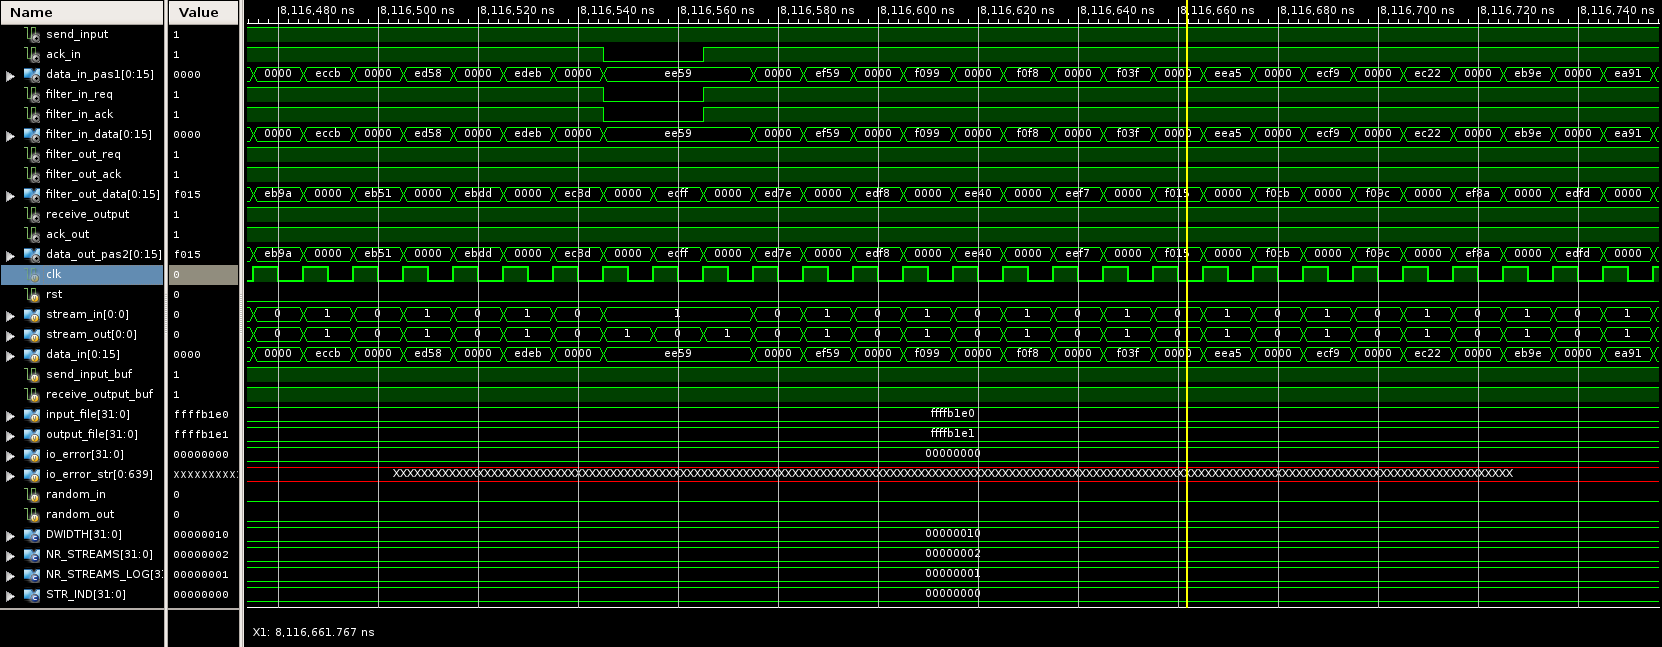
\includegraphics[width=0.7\textwidth]{images/waveforms.png}
\caption{Part of the waveforms of our design.}
\label{fig:wave}
\end{center}
\end{figure}
\FloatBarrier


\section{Appendix A: Answers to inline questions}
todo
\section{Appendix B: Verilog source code}
This appendix includes Verilog source code for the \texttt{filter.v} file in the ISE project.

\begin{verbatim}
\end{verbatim}


\end{document}
